\chapter{Những nghiên cứu liên quan}
Chương này trình bày các công trình liên quan được chúng tôi tìm hiểu trong quá trình nghiên cứu thực hiện đề tài. Các công trình này chứa các kỹ thuật và các ứng dụng có liên quan đến nội dung mà chúng tôi nghiên cứu, hoặc được chúng tôi ứng dụng vào nghiên cứu này.

\section{Dự báo nhiều bước trong dữ liệu chuỗi thời gian (multi-step ahead predictions)}
Nếu dự báo một bước trong dữ liệu chuỗi thời gian đang là một bài toán thách thức trong mạng nơ-ron học sâu, thì dự báo nhiều bước lại càng đầy thách thức hơn. Hiện nay, có nhiều cách tiếp cận để giải quyết vấn đề phức tạp này. Một nghiên cứu tổng quan của Nguyen Hoang An và các cộng sự đã so sánh các chiến lược tiếp cận hiệu quả và đang được ưa chuộng cho dự báo nhiều bước như: hồi quy, trực tiếp, kết hợp hồi quy và trực tiếp, nhiều đầu vào – nhiều đầu ra, kết hợp trực tiếp và nhiều đầu vào – nhiều đầu ra \cite{st17}.

\subsection{Chiến lược hồi quy (Recursive Strategy)}
Trong chiến lược này, một mô hình \textbf{\textit{g}} được huấn luyện để dự báo một bước.

\begin{equation}
\label{eq:12}
y_{t+1}=f(y_t,…,y_{t-d+1} )+ w \: (with \: t \in \{d,…,N-1\})
\tag{12}
\end{equation}

Khi dự báo \textit{H} bước, ta sẽ dự báo bước đầu tiên bằng cách sử dụng mô hình. Kế đến, ta sử dụng giá trị vừa mới được dự báo để  hem vào dữ liệu đầu vào cho dự báo bước kế tiếp. Ta lặp lại cho đến khi đạt được \textit{H} bước, hình \ref{fig:3-1}.

Giả sử chúng ta huấn luyện được mô hình dự báo một bước \textbf{\textit{ĝ}}. Dự báo nhiều bước sẽ có dạng sau:

\begin{equation}
\label{eq:13}
\widehat{y}_{N+h} = \left\{\begin{matrix}
\widehat{g}(y_N,...,y_{N-d+1}) & $     $if $ $ h =1 
\\ \widehat{g}(y_{N+h-1},...,y_{N+1},y_N,y_{N-d+h}) & $ $if $ $ h\in\{2,...,d\}
\\ \widehat{g}(y_{N+h-1},...,y_{N+h-d}) & $   $ if $ $ h\in\{d+1,...,H\}
\end{matrix}\right.
\tag{13}
\end{equation}

\begin{figure}[H]
    \centering
    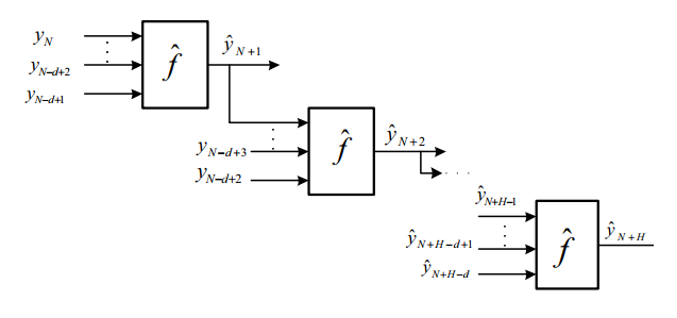
\includegraphics[scale=1.25]{./content/images/3-1.png}
    \caption{Kiến trúc chiến lược hồi quy \cite{st17}}
    \label{fig:3-1}
\end{figure}

\subsection{Chiến lược trực tiếp (Direct Strategy)}
Trong chiến lược này, ta sẽ có \textit{H} mô hình \textbf{\textit{$g_{h}$}} được huấn luyện (một cho mỗi chuỗi con) từ chuỗi thời gian, hình \ref{fig:3-2}:

\begin{equation}
\label{eq:14}
y_{t+h}=g_h (y_1,...,y_{t-d+1} )+ w \: (with \: t\in \{d,...,N-H\} \: and \: h\in\{1,...,H\})
\tag{14}
\end{equation}

Các dự báo sẽ được xác định bằng cách sử dụng \textit{H} mô hình \textbf{\textit{ĝ}} đã được huấn luyện:

\begin{equation}
\label{eq:15}
\widehat{y}_{N+h} = \widehat{g}_{h}(y_N,...,y_{N-d+1})
\tag{15}
\end{equation}

\begin{figure}[!h]
    \centering
    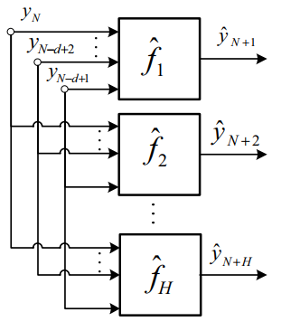
\includegraphics[scale=1.25]{./content/images/3-2.png}
    \caption{Kiến trúc chiến lược trực tiếp \cite{st17}}
    \label{fig:3-2}
\end{figure}

\subsection{Kết hợp chiến lược hồi quy và chiến lược trực tiếp (DirREC Strategy)}
Kết hợp ưu điểm của chiếc lược hồi quy và chiến lược trực tiếp. Trong chiến lược này, ta sẽ dự báo với nhiều mô hình khác nhau cho từng chuỗi con (như chiến lược trực tiếp). Và tại mỗi thời điểm, dữ liệu dự báo được sẽ được thêm vào cho dữ liệu đầu vào của bước tiếp theo (như chiến lược hồi quy), hình \ref{fig:3-3}. Tuy nhiên, có một điểm khác biệt với hai chiến lược kia, chiều dài mỗi chuỗi con sẽ không giống nhau cho từng thời điểm. Chiến lược này huấn luyện \textit{H} mô hình $\mathbf{g_h}$ từ chuỗi thời gian [$y_{1}$,…,$y_{N}$]:

\begin{equation}
\label{eq:16}
y_{t+h}=g_h(y_{t+h-1},...,y_{t+d-1} )+w \:  (with \: t\in\{d,...,N-H\} \: and \: h\in\{1,...,H\})
\tag{16}
\end{equation}

Các dự báo sẽ được xác định bằng cách sử dụng \textit{H} mô hình \textit{\textbf{ĝ}} đã được huấn luyện:

\begin{equation}
\label{eq:17}
\widehat{y}_{N+h} = \left\{\begin{matrix}
\widehat{g}(y_n,...,y_{N-d+1}) & $     $if $ $ h =1 
\\ \widehat{g}(y_{N+h-1},...,y_{N+1},y_N,y_{N-d+1}) & $ $if $ $ h\in\{2,...,H\}
\end{matrix}\right.
\tag{17}
\end{equation}

\begin{figure}[H]
    \centering
    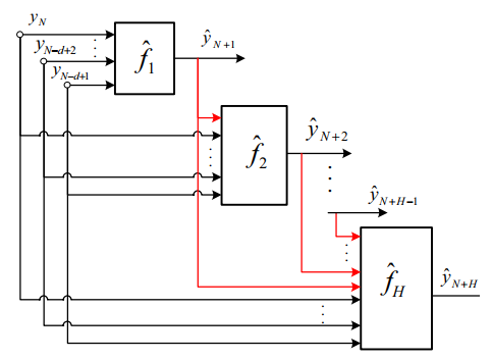
\includegraphics[scale=1.25]{./content/images/3-3.png}
    \caption{Kiến trúc kết hợp chiến lược hồi quy và trực tiếp \cite{st17}}
    \label{fig:3-3}
\end{figure}

\subsection{Chiến lược nhiều đầu vào – nhiều đầu ra (MIMO Strategy)}
Ba giải thuật được đề cập ở trên (hồi quy, trực tiếp, kết hộp hồi quy và trực tiếp) dựa trên dự báo một bước đầu ra và mô hình nhận nhiều đầu vào, nhưng chỉ cho một đầu ra.
Chiến lược nhiều đầu vào – nhiều đầu ra sẽ huấn luyện mô hình nhiều đầu ra \textbf{\textit{g}} từ chuỗi thời gian [$y_{1}$,…,$y_{N}$], hình \ref{fig:3-4}:

\begin{equation}
\label{eq:18}
[y_{t+H},...,y_{t+1}] = g(y_t,...,y_{t-d+1}) + w
\tag{18}
\end{equation}

\begin{center}
(với \textit{t} \in \{d,…,N-H\}, g:$R^{d}$→$R^{h}$ là vec-tơ giá trị hàm và \textit{w} \in \: $R^{H}$ là vec-tơ nhiễu)
\end{center}

Các giá trị dự báo sẽ được trả về trong một bước bởi mô hình nhiều đầu ra \textit{\textbf{ĝ}}:

\begin{equation}
\label{eq:19}
[\widehat{y}_{t+H},...,\widehat{y}_{t+1}] = \widehat{g}(y_N,...,y_{N-d+1})
\tag{19}
\end{equation}

\begin{figure}[H]
    \centering
    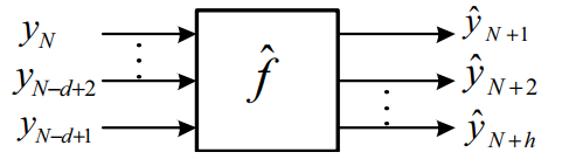
\includegraphics[scale=0.75]{./content/images/3-4.png}
    \caption{Kiến trúc chiến lược nhiều đầu vào – nhiều đầu ra \cite{st17}}
    \label{fig:3-4}
\end{figure}

\subsection{Kết hợp chiến lược trực tiếp và chiến lược nhiều đầu vào - nhiều đầu ra (DirMO Strategy)}
Với chiến lược này, ta dự đoán từng đoạn \textit{H} trong những khối. Với mỗi khối, ta sử dụng chiến lược nhiều đầu vào nhiều đầu ra, hình \ref{fig:3-5}. Vì thế, dự báo \textit{H} bước sẽ được chia thành \textit{n} dự báo nhiều đầu ra (\textit{n=H/s}), với mỗi đầu ra có kích thước \textit{s} (\textit{s} \in \{1,..,\textit{H}\}).

Chiến lược sẽ huấn luyện \textit{n} mô hình $\mathbf{g_{p}}$ từ chuỗi thời gian [$y_{1}$,…,$y_{N}$]:

\begin{equation}
\label{eq:20}
[y_{t+p+s},...,y_{t+(p-1)*s+1}]= g_p(y_t,...,y_{t-d+1}) + w
\tag{20}
\end{equation}

\begin{center}
(với \textit{t} \in \{d,…,N-H\}, \textit{p} \in \{1,..,\textit{N}\}, g:$R^{d}$→$R^{s}$ là vec-tơ giá trị hàm với \textit{s} > 1 và \textit{w} \in \: $R^{H}$ là vec-tơ nhiễu)
\end{center}

\begin{figure}[H]
    \centering
    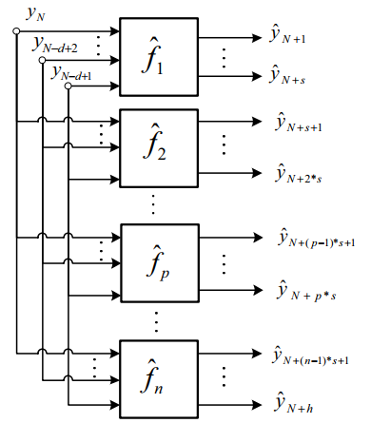
\includegraphics[scale=1.25]{./content/images/3-5.png}
    \caption{Kiến trúc kết hợp chiến lược trực tiếp và nhiều đầu vào–nhiều đầu ra \cite{st17}}
    \label{fig:3-5}
\end{figure}

\section{Giải thuật HOT SAX}
Lin và các cộng sự \cite{st6} \cite{st34} đã đề xuất một phương pháp rời rạc hóa có tên là \textit{xấp xỉ gộp ký hiệu hóa} (symbolic aggregate approximation – SAX) mà dựa trên phương pháp thu giảm số chiều PAA \cite{st9} \cite{st33} và giả sử dữ liệu thu giảm số chiều đã đươc chuẩn hóa. SAX là quá trình ánh xạ biểu diễn PAA của chuỗi thời gian thành một chuỗi ký tự rời rạc. Gọi \textit{a} là kích thước của bộ ký hiệu mà được dùng để rời rạc hóa chuỗi thời gian. Để ký hiệu hóa chuỗi thời gian chúng ta phải tìm thấy các trị (điểm ngắt) sau đây:

\begin{equation}
\label{eq:21}
\beta_1,\beta_2,...,\beta_{a-1} \:  with \: \beta_1 < \beta_2 <...< \beta_{a-1}
\tag{21}
\end{equation}

Sử dụng những giá trị này, chuỗi thời gian $\overline{T}$ = $\overline{t_1}$,...,$\overline{t_w}$ sẽ được rời rạc hoá thành tràng ký hiệu \textit{C} = $c_{1}$,$c_{2}$,…,$c_{w}$, hình \ref{fig:3-7}. Mỗi đoạn $\overline{t_i}$ sẽ được mã hoá thành ký hiệu $c_{i}$ dùng công thức sau:

\begin{equation}
\label{eq:22}
c_i=\left\{\begin{matrix}
c_1 $ $ \overline{t_i} \leq \beta_1
\\ c_a $ $ \overline{t_i} >  \beta_{a-1}
\\ c_k $ $ \beta_{k-1} < \overline{t_i} \leq \beta_k
\end{matrix}\right.
\tag{22}
\end{equation}

\begin{figure}[H]
    \centering
    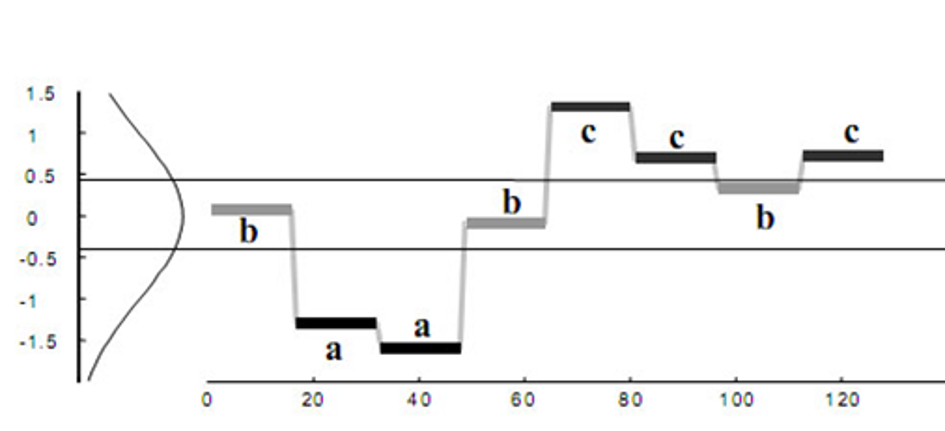
\includegraphics[scale=0.75]{./content/images/3-7.png}
    \caption{Một chuỗi thời gian được biến đổi PAA rồi mã hóa thành các ký hiệu \cite{st12}}
    \label{fig:3-7}
\end{figure}

Chúng ta chú ý rằng dữ liệu chuỗi thời gian thường có phân bố xác xuất Gauss. Để có một xác xuất bằng nhau (1/\textit{a}) cho mỗi ký hiệu, ta phải chọn trị điểm ngắt $\beta_{i}$ dựa trên bảng xác xuất của phân bố Gauss.

Dữ liệu chuỗi thời gian sẽ được thu giảm số chiều qua biến đổi PAA. Ngoài ra, HOT SAX cũng áp dụng một giải thuật biến đổi khác để đạt được một biểu diễn SAX rời rạc. Lưu ý là biểu diễn SAX yêu cầu dữ liệu phải thoả mãn phân phối Gauss. Để tìm được những đoạn bất thường với độ dài \textit{n} trên chuỗi dữ liệu thời gian, trước tiên HOT SAX sử dụng một cửa sổ trượt với độ dài \textit{n} dọc theo chuỗi thời gian \textit{T}, lấy một cách tuần tự, mã hoá chúng vào chuỗi ký tự (gọi là từ SAX) và vị trí chúng trong bảng được tham chiếu theo chuỗi thời gian gốc. Một khi có được thứ tự của danh sách các ký tự SAX, HOT SAX sẽ lưu trữ chúng dưới dạng cấu trúc cây, với nốt lá chứa danh sách số lần xuất hiện của tất cả từ SAX. HOT SAX dựa trên ba yếu tố quan trọng: độ dài \textit{n} của các chuỗi bất thường, số lượng \textit{$\alpha$} của tập hợp ký tự SAX, độ dài từ SAX.

Để thoát khỏi các vòng lặp sớm, HOT SAX áp dụng hai kỹ thuật sau. (a) Với vòng lặp bên ngoài, chuỗi con có khoảng cách lớn hơn tới lân cận gần nhất của nó sẽ được ưu tiên chọn để so sánh. Những chuỗi con này sẽ được tham chiếu tới các nốt là có số lượng xuất hiện thấp. (b), Với vòng lặp ở bên trong, chuỗi con với khoảng cách nhỏ hơn đến đối tượng đang được tham chiếu sẽ được ưu tiên để so sánh. Những chuỗi con này sẽ tham chiếu tới cùng nốt lá với đối tượng đang được tham chiếu.

\section{Mạng LSTM xếp chồng trong phát hiện chuỗi con bất thường}
Mạng LSTM được chứng mình rất hữu dụng cho dữ liệu chuỗi thời gian có tính phụ thuộc xa. Và việc sử dụng mạng nơ-ron học sâu LSTM xếp chồng có thể giúp học các biểu diễn mới ở mức trừu tượng cao hơn và huấn luyện nhanh hơn với số nơ-ron mỗi tầng ẩn thưa hơn. Năm 2015, Malhotra và cộng sự đã xây dựng mạng nơ-ron học sâu LSTM xếp chồng để dự báo, và kết quả dự báo lỗi được mô hình hóa vào một phân phối Gauss đa biến \cite{st14}.

\begin{figure}[H]
    \centering
    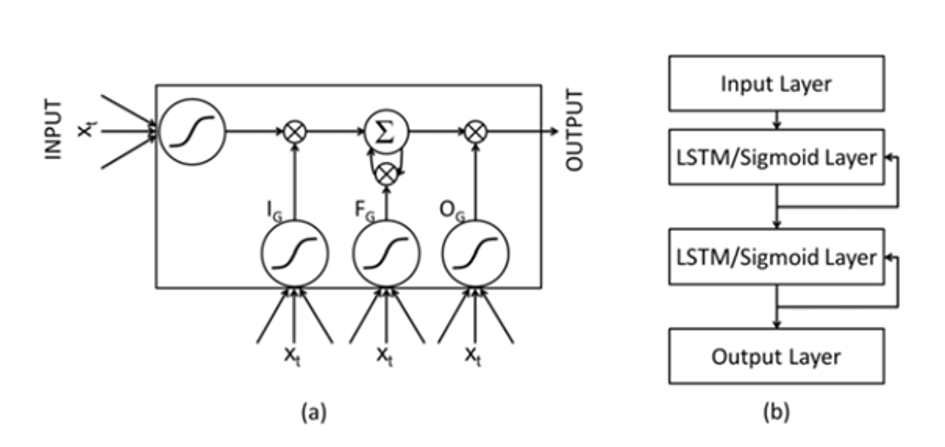
\includegraphics[scale=0.75]{./content/images/3-8.png}
    \caption{(a) LSTM cell (b) Kiến trúc LSTM xếp chồng \cite{st14}}
    \label{fig:3-8}
\end{figure}

Trong nghiên cứu này, Malhotra và cộng sự đã huấn luyện mạng nơ-ron học sâu LSTM xếp chồng (như hình \ref{fig:3-8}) để học dữ liệu chuỗi thời gian bình thường, và nhờ đó ta có thể xác định những sai lệch so với dữ liệu bình thường mà không cần tiền xử lý hoặc cửa sổ trượt.

Tập dữ liệu sẽ được chia thành các \textit{tập huấn luyện} (training set), \textit{tập kiểm thử} (validation set) và \textit{tập kiểm tra} (test set). Mạng nơ-ron học sâu LSTM xếp chồng sẽ được huấn luyện bằng tập huấn luyện. Trong khi tập kiểm thử sẽ được sử dụng trong lúc huấn luyện để kiểm tra các trọng số của mô hình.

Tiếp đến, công việc phát hiện chuỗi con bất thường sẽ sử dụng phân phối dự báo lỗi. Giả sử chuỗi thời gian  \textit{X} = \{$x^{(1)}$,…,$x^{(n)}$\}, với $x^{(t)}$ \in \ $R^{m}$ là một vec-tơ \textit{m}-chiều \{$x_{1}^{(t)}$,$x_{2}^{(t)}$,…,$x_{m}^{(t)}$\}, với một dự báo có chiều dài \textit{l} của mỗi \textit{d} chiều của $x^{(t)}$ $\in$ \textit{X}, trong khi \textit{l} < \textit{t} < \textit{n} - \textit{l}. Ta có thể xác định một vec-tơ sai số $e^{(t)}$ cho $x^{(t)}$, $e^{(t)}=[e_{11}^{(t)}$,…,$e_{1l}^{(t)}$,…,$e_{d1}^{(t)}$,…,$e_{dl}^{(t)}$]. Mạng nơ-ron học sâu LSTM xếp chồng được huấn luyện trên tập huấn luyện sẽ được dùng để tính toán vec-tơ sai số cho mỗi điểm dữ liệu trên tập kiểm thử và kiểm tra. Và những vec-tơ sai số này sẽ được mô hình hóa vào một phân phối Gauss đa biến $\mathcal{N}$ = $\mathcal{N}$($\mu$, $\Sigma$). Hàm phân phối $p^{(t)}$ cho giá trị $\mathcal{N}$ tại $e^{(t)}$ được xác định bằng $\mu$ và $\Sigma$. Từ đó, một điểm dữ liệu $x^{(t)}$ được phân loại là bất thường nếu $p^{(t)}$ < $\tau$ và ngược lại sẽ được phân loại là bình thường. Tập huấn luyện và kiểm thử được dùng để học $\tau$ bằng cách tối ưu $F_\beta$-score.

Mô hình của Malhotra và các cộng sự bước đầu đã mang lại kết quả bước đầu khả quan, cũng như đưa ra nhiều hướng đi mới cho các nghiên cứu sau này. Nhưng điểm bất lợi trong nghiên cứu của Malhotra và các cộng sự là nghiên cứu chỉ so sánh việc sử dụng LSTM với RNN, trong khi hai mô hình này có tính chất giống nhau nên không nêu rõ được sự hiệu quả của hướng tiếp cận này. Bên cạnh đó, Malhotra và các cộng sự không so sánh với các hướng tiếp cận tiêu biểu khác trong các công trình đi trước, nên dẫn đến việc đánh giá tính hiệu quả của mô hình không được rõ ràng.

\section{Kết hợp mạng nơ-ron học sâu và mô hình xác suất truyền thống}
Năm 2018, Buda và các cộng sự đã có một hướng đi táo bạo, bằng việc kết hợp mạng nơ-ron học sâu và phương pháp xác suất thống kê truyền thống trong một mô hình để dự báo bất thường cho dữ liệu chuỗi thời gian \cite{st15}. Với sự kết hợp này, mô hình hoạt động tốt cho cả tập dữ liệu tuyến tính và tập dữ liệu không ổn định, hỗn loạn. Buda và các cộng sự đặt tên cho mô hình này là DeepAD (như hình \ref{fig:3-9}).

\begin{figure}[H]
    \centering
    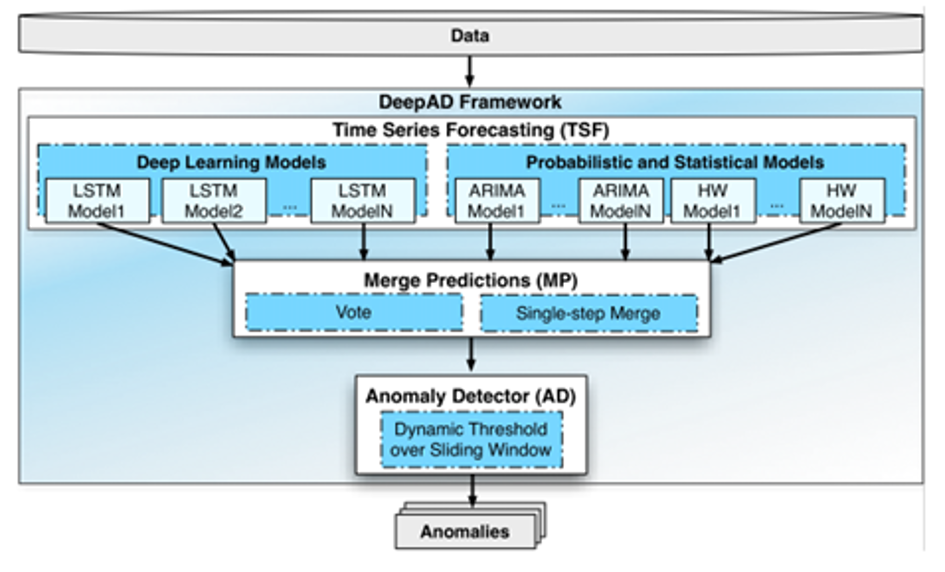
\includegraphics[scale=0.95]{./content/images/3-9.png}
    \caption{Kiến trúc mô hình kết hợp mạng học sâu và mô hình xác suất \cite{st15}}
    \label{fig:3-9}
\end{figure}

\textbf{Time Series Forecasting (TSF):} Với sự kết hợp giữa mạng học sâu và mô hình xác suất thống kê, DeepAD sử dụng các kiến trúc khác nhau để học những hành vi bình thường của dữ liệu, cũng như sử dụng nhiều kiến trúc trong dự báo.

\textbf{Merge Predictions (MP):} với \textit{Single-step merge}, DeepAD kết hợp dự báo của nhiều mô hình để có kết quả đầu ra chính xác nhất. Theo đó, mô hình sẽ chọn kiến trúc có độ sai số thấp nhất tại mỗi mốc thời gian. Với \textit{Vote}, chúng ta sẽ sử dụng kiến trúc phù hợp với đặc tính dữ liệu đầu vào. Theo đó, mô hình sẽ chọn kiến trúc cung cấp độ sai số thấp nhất trên tập dữ liệu đầu vào.

\textbf{Anomaly Detector (AD):} dựa vào sai số giữa giá trị dự báo và giá trị thực tế, DeepAD tính toán một giá trị ngưỡng động tại mỗi thời điểm. Với cách tiếp cận này, mô hình sẽ không phụ thuộc vào giá trị ngưỡng cố định.

Giải thuật \textit{Algorithm 1} mô tả cách thức xác định chuỗi con bất thường. Theo đó, nếu giá trị bình phương sai số của dự báo cao hơn 10 lần giá trị chuẩn của bình phường các dự báo trước đó, mô hình sẽ cân nhắc đó là bất thường. Do đó, giá trị ngưỡng và bình phương sai số luôn được thay đổi để đáp ứng với giá trị mới và tăng độ chính xác.

\begin{table}[H]
\centering
\begin{tabular}{l}
\hline
\textbf{Algorithm 1:} isAnomaly(\textit{actualValue}, \textit{pastValues}, \textit{squaredErrors}, \\\textit{predictedValue}, \textit{look\_back}, \textit{slidingWindow})\\
\hline
\begin{tabular}[l]{@{}l@{}}
\textbf{1} \textit{scaler} \leftarrow \textbf{MinMaxScaler}(\textit{feature\_range} = (0,1)));
\\\textbf{2} \textbf{//Rescale errors from sliding window for dynamic threshold fitiing;}
\\\textbf{3} \textit{scaledSErrors} \leftarrow \textit{scaler}\textbf{.fitTransform}(\textit{squaredErrors}[-\textit{slidingWindow} :]);
\\\textbf{4} \textbf{//Computer dynamic threshold as 10 times standard deviation;}
\\\textbf{5} \textit{dynamic\_thresh} \leftarrow 10 * \textbf{numpy.std}(\textit{scaledErrors});
\\\textbf{6} \textbf{//Caculate squared error and apply transformation on current error}
\\$       $ \textit{crtSError} \leftarrow (\textit{actualValue} - \textit{predictedValue}) \wedge 2;
\\\textbf{7} \textit{crtScaledSError} \leftarrow \textit{scaler}\textbf{.transform}(\textit{crtSError});
\\\textbf{8} \textbf{//If current error bigger than dynamic threshold signal return} \textit{True};
\\\textbf{9} \textbf{if } \textit{crtScaledSError} \geq \textit{dynami\_thresh } \textbf{then return } \textit{True };
\\\textbf{10} \textbf{//Otherwise add non scaled squared error to the queue};
\\\textbf{11} \textit{squaredErrors} \leftarrow \textit{squaredErrors}\textbf{.put}(\textit{crtSError});
\\\textbf{12} \textbf{return } \textit{False} \\
\end{tabular}
\\\hline
\end{tabular}
\end{table}

Mô hình này mở ra một hướng đi mới về bài toán dự báo và phát hiện bất thường, nhưng nó lại quá phức tạp trong việc gộp nhiều mô hình. Mặt khác, nghiên cứu này chỉ đưa ra hướng đi mới và không so sánh với các giải thuật đã được nghiên cứu trước đó, dẫn đến chưa làm nổi bật được hiệu quả của sự kết hợp này.

\section{Dự báo dữ liệu và chỉnh sửa bất thường dựa trên mạng LSTM}
Năm 2020, với sự bùng nổ của các mạng nơ-ron học sâu, đặc biệt là mạng nơ-ron học sâu LSTM. Ngoài việc sử mạng nơ-ron học sâu LSTM trong công tác dự báo, Lei Zhang và cộng sự đã ứng dụng vào công tác chỉnh sửa bất thường. Với dữ liệu được dự báo từ mạng LSTM, Lei Zhang và cộng sự đã sử dụng dữ liệu dự báo này để phát hiện bất thường và chỉnh sửa bất thường và đưa dữ liệu này vào tái huấn luyện mô hình \cite{st31}.
Đi sâu vào công tác dự báo, dữ liệu được dự báo sẽ dựa vào dữ liệu trong lịch sử. Thông thường trước khi tiến hành dự báo, một lượng lớn dữ liệu trong lịch sử sẽ được thu thập. Các giá trị dữ liệu này sẽ đại diện cho đặc tính của dữ liệu, dữ liệu càng bao quát thì độ chính xác dự báo càng cao. Dữ liệu sẽ được tiền xử lý trước khi đưa vào huấn luyện mạng LSTM. Sau đó, mô hình sẽ được huấn luyện với các thông số thích hợp. Sau khi mô hình được đào tạo, giá trị dự báo có thể nhận được bằng cách đưa dữ liệu lịch sử vào mô hình LSTM đã đào tạo. Quá trình đào tạo hoàn chỉnh về \textit{dự báo phụ tải} (load forecasting) sử dụng LSTM được thể hiện trong hình \ref{fig:3-11}.

\begin{figure}[H]
    \centering
    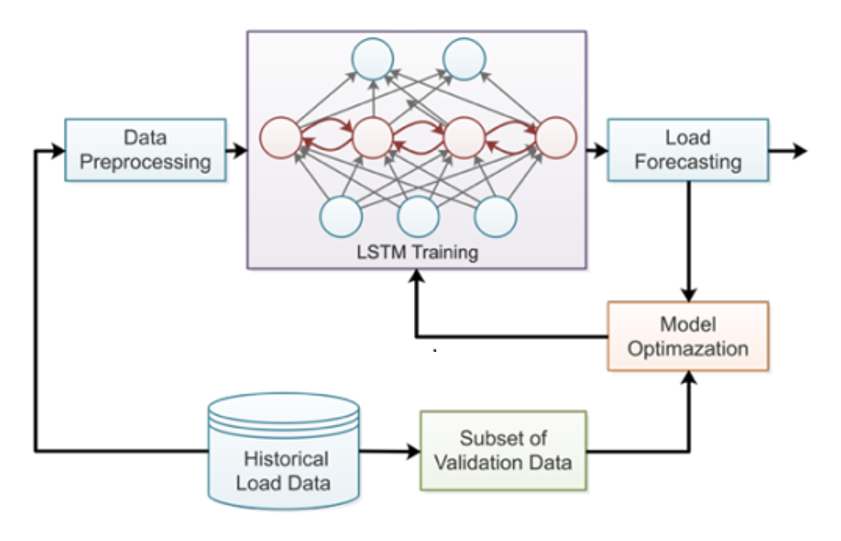
\includegraphics[scale=0.95]{./content/images/3-11.png}
    \caption{Quy trình huấn luyện và dự báo bằng mạng LSTM \cite{st31}}
    \label{fig:3-11}
\end{figure}

Dữ liệu bất thường sẽ ảnh hưởng tiêu cực đến kết quả dự báo vì nó phá hủy các đặc trưng của dữ liệu và mô hình dự báo không còn nhận ra mối quan hệ giữa các dữ liệu. Bởi vì mạng nơ-ron học sâu LSTM khác biệt với các mô hình khác vì sự tương thích mẽ mạnh mẽ của nó trên dữ liệu chuỗi thời gian, một số lượng nhỏ bất thường sẽ không có tác động nghiêm trọng đến kết quả dự báo. Do đó, kết quả dự báo có thể được sử dụng để xác định sự bất thường và sửa chữa nó bằng các kết quả dự báo. Theo Lei Zhang và cộng sự, dữ liệu bất thường phổ biến có thể được phân loại thành 3 loại: dữ liệu có giá trị rỗng, dữ liệu không đủ, dữ liệu có giá trị quá cao hoặc quá thấp.

Thực hiện dự báo trong các tình huống có dữ liệu bất thường. Sau đó, Kết quả dự báo được so sánh với giá trị của dữ liệu gốc tại cùng thời điểm để xác định xem sự bất thường có cần sửa chữa hay không. Cuối cùng, các điểm dữ liệu bất thường đã được chỉnh sửa sẽ được đưa vào để huấn luyện lại mô hình LSTM. Sơ đồ hoàn chỉnh của cách tiếp cận được đề xuất được miêu tả trong hình \ref{fig:3-12}.

\begin{figure}[H]
    \centering
    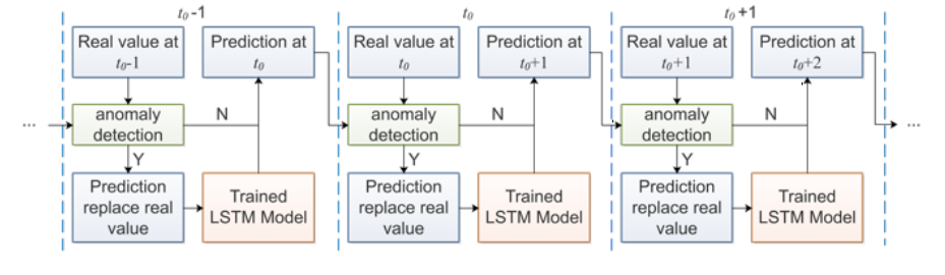
\includegraphics[scale=1.05]{./content/images/3-12.png}
    \caption{Sơ đồ hoàn chỉnh của phương pháp tiếp cận được đề xuất \cite{st31}}
    \label{fig:3-12}
\end{figure}

Một trong những kết quả của việc chỉnh sửa bất thường đã được Lei Zhang và các cộng sự thực hiện như hình \ref{fig:3-13}.

\begin{figure}[H]
    \centering
    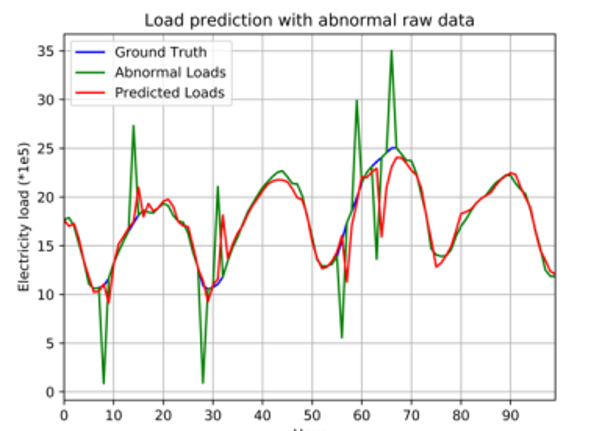
\includegraphics[scale=1.25]{./content/images/3-13.png}
    \caption{Kết quả dự báo dựa trên dữ liệu chưa được hiệu chỉnh \cite{st31}}
    \label{fig:3-13}
\end{figure}

Dễ dàng nhận thấy, nếu sử dụng giá trị dự báo từ mô hình LSTM để chỉnh sửa cho những bất thường thì bộ dữ liệu này miêu tả đúng hơn về mối liên quan của các điểm dữ liệu. Sau đó, dùng bộ dự liệu đã được chỉnh sửa để đưa vào huấn luyện mô hình LSTM, và kết quả huấn luyện sẽ đạt kết quả tốt hơn nếu ta chỉ sử dụng bộ dữ liệu ban đầu.

Hướng tiếp cận này đã lần nữa khẳng định khả năng làm việc tốt của mạng nơ-ron học sâu LSTM trên các bộ dữ liệu chuỗi thời gian, và mở ra thêm một ứng dụng của công tác phát hiện bất thường bằng phương pháp dự báo, một phương pháp đang ngày càng được nhiều nhà nghiên cứu sử dụng.

\section{Kết luận}
Qua quá trình nghiên cứu tìm hiểu các công trình liên quan đến bài toán chuỗi thời gian nói chung và bài toán phát hiện bất thường nói riêng, chúng tôi thấy rằng đây là lĩnh vực nhiều nhà nghiên cứu quan tâm và áp dụng nhiều phương pháp để giải quyết từ những phương pháp thống kê truyền thống cho đến những mô hình học sâu phức tạp. Với sự phát triển mạnh mẽ của phần cứng, các mô hình học sâu đã có những bùng nổ trong những năm gần đây. Trong đó, RNN và LSTM với thiết kế để xử lý dữ liệu dạng chuỗi, thể hiện được sự tương hỗ của dữ liệu được áp dụng thành công vào nhiều bài toán như dịch máy, nhận diện giọng nói, chuyển đổi chữ thành giọng nói và ngược lại,.... Điều này thúc đẩy chúng tôi sử dụng phương pháp phát hiện bất thường bằng dự báo và kiến trúc LSTM để thực hiện nghiên cứu này.